\documentclass[a4paper,10pt,twoside]{article}

\usepackage[top=1in, bottom=1in, left=1in, right=1in]{geometry}
\usepackage[utf8]{inputenc}
\usepackage[spanish,es-ucroman,es-noquoting]{babel}
\usepackage{setspace}
\usepackage{fancyhdr}
\usepackage{lastpage}
\usepackage{amsmath}
\usepackage{amsfonts}
\usepackage{verbatim}
\usepackage{graphicx}

%Configuraciones de tp2
\usepackage{amssymb}
\usepackage{url}

% Evita que el documento se estire verticalmente para ocupar
% el espacio vacío en cada página.
\raggedbottom


%%%%%%%%%% Configuración de Fancyhdr - Inicio %%%%%%%%%%
\pagestyle{fancy}
\thispagestyle{fancy}
\lhead{Trabajo Práctico 2, Organización del Computador II}
\rhead{Capra, Lovisolo, Petaccio}
\renewcommand{\footrulewidth}{0.4pt}
\cfoot{\thepage /\pageref{LastPage}}

\fancypagestyle{caratula} {
   \fancyhf{}
   \cfoot{\thepage /\pageref{LastPage}}
   \renewcommand{\headrulewidth}{0pt}
   \renewcommand{\footrulewidth}{0pt}
}
%%%%%%%%%% Configuración de Fancyhdr - Fin %%%%%%%%%%


\begin{document}
%%%%%%%%%%%%%%%%%%%%%%%%%%%%%%%%%%%%%%%%%%%%%%%%%%%%%%%%%%%%%%%%%%%%%%%%%%%%%%%
%% Carátula                                                                  %%
%%%%%%%%%%%%%%%%%%%%%%%%%%%%%%%%%%%%%%%%%%%%%%%%%%%%%%%%%%%%%%%%%%%%%%%%%%%%%%%


\thispagestyle{caratula}

\begin{center}


\includegraphics[height=2cm]{DC.png} 
\hfill

\includegraphics[height=2cm]{UBA.jpg} 

\vspace{2cm}

Departamento de Computación,\\
Facultad de Ciencias Exactas y Naturales,\\
Universidad de Buenos Aires

\vspace{1cm}

\begin{spacing}{2.5}
\begin{Huge}
Reducción de ruido con \\Transformada Discreta del Coseno
\end{Huge}
\end{spacing}

\vspace{1cm}

Trabajo Práctico 1, \\
Métodos Numéricos, \\
Primer Cuatrimestre de 2013

\vspace{6cm}

\begin{tabular}{|c|c|c|}
\hline
Apellido y Nombre & LU & E-mail\\
\hline
María Candela Capra Coarasa & 234/11 & canduh\_27@hotmail.com\\
Leandro Lovisolo            & 645/11 & leandro@leandro.me\\
Lautaro José Petaccio       & 443/11 & lausuper@gmail.com\\
\hline
\end{tabular}

\end{center}
\vspace{1cm}

\textbf{Resumen:} \\
Se aplican distintos métodos para agregar ruido a señales sonoras e imágenes para luego, utilizando la Transformada Discreta del Coseno, plantear y sacar conclusiones sobre la eficiencia de varias técnicas de reducción del ruido agregado.

\textbf{Palabras claves:}
Reducción, ruido, DST, sonido, imágenes, frecuencia.
\newpage

%%%%%%%%%%%%%%%%%%%%%%%%%%%%%%%%%%%%%%%%%%%%%%%%%%%%%%%%%%%%%%%%%%%%%%%%%%%%%%%
%% Índice                                                                    %%
%%%%%%%%%%%%%%%%%%%%%%%%%%%%%%%%%%%%%%%%%%%%%%%%%%%%%%%%%%%%%%%%%%%%%%%%%%%%%%%


\tableofcontents

\newpage

%%%%%%%%%%%%%%%%%%%%%%%%%%%%%%%%%%%%%%%%%%%%%%%%%%%%%%%%%%%%%%%%%%%%%%%%%%%%%%%
%% Introducción Teórica                                                      %%
%%%%%%%%%%%%%%%%%%%%%%%%%%%%%%%%%%%%%%%%%%%%%%%%%%%%%%%%%%%%%%%%%%%%%%%%%%%%%%%


\section{Introducción Teórica}

En este trabajo exploramos un conjunto de métodos basados en la Transformada Discreta del Coseno para eliminar ruidos aperiódicos sobre muestras de señales de una y dos dimensiones (ejemplo: audio e imágenes, respectivamente).

La Transformada Discreta del Coseno, de ahora en más DCT, permite expresar un vector en $\mathbb{R}^n$ como combinación lineal de vectores de la forma $\{(cos(0 * t_0), \ldots cos(0 * t_{n-1})), \ldots (cos(n-1 * t_0), \ldots cos(n-1 * t_{n-1})) \}$, donde n es el tamaño de la muestra y $t_i = (i + \frac{1}{2})\frac{\pi}{n}$. Gráficamente, se puede interpretar este cambio de base como la escritura de la muestra como una suma de cosenos de distintas frecuencias, donde las coordenadas del vector transformado son coeficientes que determinan la amplitud de cada coseno, y se presentan ordenados de menor a mayor frecuencia.

En el caso de señales bidimensionales representadas con matrices $\mathbb{R}^{n \times n}$, la matriz transformada obtenida es análoga al caso unidimensional, en la que se pueden obtener los coeficientes ordenados de menor a mayor frecuencia recorriendo las coordenadas diagonalmente de derecha a izquierda y arriba a abajo, partiendo de la coordenada superior izquierda.

Los tipos de ruido aplicados a las muestras son aditivo e impulsivo, descritos a continuación:

\begin{description}

\item[Ruido aditivo:]

Suma a cada elemento de la muestra una variable aleatoria con distribución normal, con media cero y distintas varianzas de acuerdo al experimento.

\item[Ruido impulsivo:]

Reemplaza cada elemento de la muestra por máx o mín con probabilidad p, donde máx y mín representan el valor máximo y mínimo que adquieren los elementos de la muestra, y p variable de acuerdo al experimento.

\end{description}



% \textbf{Transformada Discreta del Coseno}
% En el caso real, expresa una función $f()$ determinada utilizando una base formada
% por $\{cos(0x),cos(x),cos(2x),...,cos((n-1)x)\}$.

% En el caso discreto es un cambio de base, dónde la base usada se compone de cosenos discretizados a distintas frecuencias


%%%%%%%%%%%%%%%%%%%%%%%%%%%%%%%%%%%%%%%%%%%%%%%%%%%%%%%%%%%%%%%%%%%%%%%%%%%%%%%
%% Desarrollo                                                                %%
%%%%%%%%%%%%%%%%%%%%%%%%%%%%%%%%%%%%%%%%%%%%%%%%%%%%%%%%%%%%%%%%%%%%%%%%%%%%%%%


\section{Desarrollo}

\subsection{Atenuar}

\subsubsection{Ruido aditivo en audio}

Muestra ramp1234.txt, varianza 10.

PSNR de la muestra con ruido agregado: 22.5536

PSNR de la muestra luego de aplicar el método: 25.0304

\begin{center}
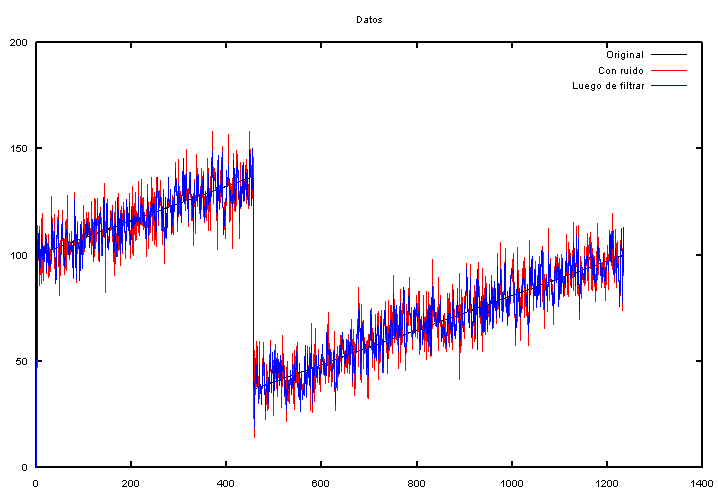
\includegraphics[width=15cm]{graficos/ramp_aditivo_atenuar_muestra.png} 
\end{center}

\begin{center}
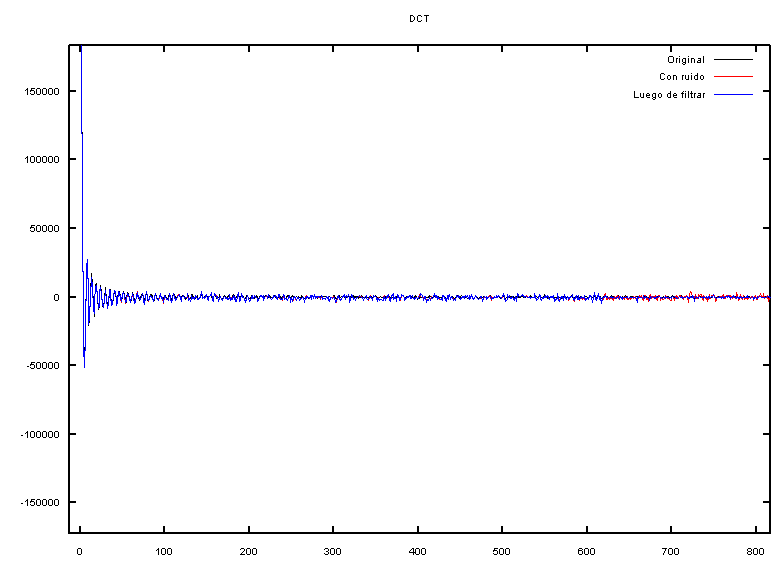
\includegraphics[width=15cm]{graficos/ramp_aditivo_atenuar_dct.png} 
\end{center}


\subsubsection{Ruido impulsivo en audio}

Muestra dopp512.txt, varianza 10.

PSNR de la muestra con ruido agregado: 16.2445

PSNR de la muestra luego de aplicar el método: 18.2166

\begin{center}
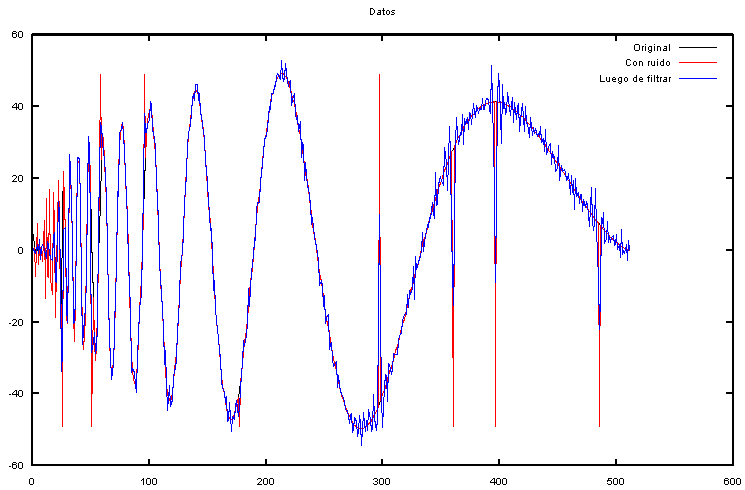
\includegraphics[width=15cm]{graficos/dopp_impulsivo_atenuar_muestra.png} 
\end{center}

\begin{center}
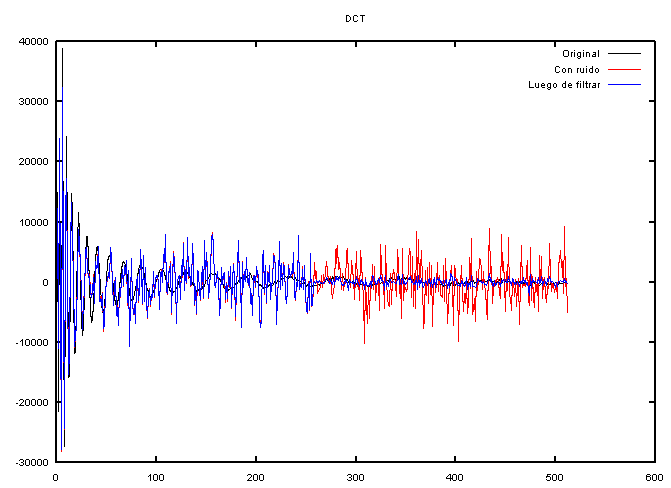
\includegraphics[width=15cm]{graficos/dopp_impulsivo_atenuar_dct.png} 
\end{center}





% \subsection{Generación de ruidos}
% Implementamos el ruido aditivo e impulsivo tanto para imágenes como para sonido.
% \subsubsection{Ruido aditivo}
% La implementación agrega ruido aditivo según la distribución probabilística normal pudiendo variarse su media y varianza para generar diferente cantidad de ruido.

% Este ruido generalmente altera todas las frecuencias de la señal por igual variando su intensidad según los cambios en la varianza.

% \subsubsection{Ruido impulsivo}
% La implementación recorre la señal o la imágen y cambia sus valores por su máximo o mínimo según un valor $p$ asociado a los valores aleatorios obtenidos mediante una distribución probabilística uniforme entre $[0,1]$. Si el valor aleatorio es $< p$ entonces se impulsa la señal al máximo, si es $\geq p $ se impulsa al mínimo, y si cae entre ellos la señal queda intacta.

% \subsection{Eliminación de ruido}
% Implementamos y probamos los métodos de eliminación de ruido \"atenuar\" y \"umbralizar\" descriptos a continuación sobre intervalos, ya que, en las pruebas realizadas, se consiguieron mejoras en las señales en su aplicación a intervalos específicos.

% En el caso de imágenes, el intervalo se tiene en cuenta según su recorrido en forma diagonal, abarcando desde los cosenos con más baja frecuencia hasta los de más alta.

% \subsubsection{Atenuar intervalo}
% Este método de reducción de ruido, multiplica a un intervalo de la señal por una constante k de doble precisión de punto flotante.

% Para el caso de un k menor que uno, la señal se reduce, siendo útil para reducir incrementos de amplitudes en frecuencias.

% \subsubsection{Umbralizar intervalo}
% El método recorre un intervalo la señal, buscando y poniendo en 0 los valores que sean menores al valor absoluto de una constante k que recibe como parámetro.

% La idea de su implementación es utilizarse para poder umbralizar ciertas frecuencias que no suelen pasar de un valor determinado, pudiendo atenuar el ruido de la señal.




%%%%%%%%%%%%%%%%%%%%%%%%%%%%%%%%%%%%%%%%%%%%%%%%%%%%%%%%%%%%%%%%%%%%%%%%%%%%%%%
%% Resultados                                                                %%
%%%%%%%%%%%%%%%%%%%%%%%%%%%%%%%%%%%%%%%%%%%%%%%%%%%%%%%%%%%%%%%%%%%%%%%%%%%%%%%


\section{Resultados}
Pendiente.

%%%%%%%%%%%%%%%%%%%%%%%%%%%%%%%%%%%%%%%%%%%%%%%%%%%%%%%%%%%%%%%%%%%%%%%%%%%%%%%
%% Discusión                                                                 %%
%%%%%%%%%%%%%%%%%%%%%%%%%%%%%%%%%%%%%%%%%%%%%%%%%%%%%%%%%%%%%%%%%%%%%%%%%%%%%%%


\section{Discusión}
Pendiente.

%%%%%%%%%%%%%%%%%%%%%%%%%%%%%%%%%%%%%%%%%%%%%%%%%%%%%%%%%%%%%%%%%%%%%%%%%%%%%%%
%% Conclusiones                                                              %%
%%%%%%%%%%%%%%%%%%%%%%%%%%%%%%%%%%%%%%%%%%%%%%%%%%%%%%%%%%%%%%%%%%%%%%%%%%%%%%%


\section{Conclusiones}
Pendiente.

%%%%%%%%%%%%%%%%%%%%%%%%%%%%%%%%%%%%%%%%%%%%%%%%%%%%%%%%%%%%%%%%%%%%%%%%%%%%%%%
%% Apéndice A: Enunciado del Trabajo Práctico                                %%
%%%%%%%%%%%%%%%%%%%%%%%%%%%%%%%%%%%%%%%%%%%%%%%%%%%%%%%%%%%%%%%%%%%%%%%%%%%%%%%

\newpage

\section{Apéndice A: Enunciado del Trabajo Práctico}
\parskip = 10pt

\newcommand{\real}{\mathbb{R}}

{\bf Introducci\'on}

La Transformada Discreta del Coseno  (DCT, por sus siglas en ingl\'es) es una herramienta que nos permite representar cualquier se\~nal en el plano de las frecuencias. Dado que es utilizada por el est\'andar de compresi\'on de im\'agenes JPEG y formato de video MPEG, se encuentra implementada en m\'as lugares de lo que pensamos: en cada c\'amara digital o tel\'efono m\'ovil. 
La DCT no solo tiene aplicaciones al mundo de la compresi\'on (donde los valores transformados pueden ser codificados de forma eficiente), sino tambi\'en al procesamiento: el an\'alisis de qu\'e frecuencias est\'an presentes en las se\~nales es esencial en ciertos contextos de aplicaci\'on.

La idea intuitiva de esta transformada, en el plano continuo, consiste en representar una funci\'on $f: \mathbb{R} \rightarrow \mathbb{R}$ en la base de funciones $\mathcal{B}=\{1, \cos(x), \cos(2x),...\}$.
En el plano discreto, la DCT se corresponde a un cambio de base: cada una de las funciones de la base $\mathcal{B}$ se discretiza en ciertos puntos pasando a ser una base de vectores en $\mathbb{R}^n$, (donde $n$ es la dimensi\'on del vector o se\~nal a transformar).
Es decir, dado un vector o se\~nal $x\in\mathbb{R}^n$ existe una matriz $M\in\mathbb{R}^{n\times n}$ de cambio de base que define la transformada DCT, donde $y=Mx$ es el vector o se\~nal transformado al espacio de frecuencias por la DCT (ver ap\'endice \ref{sec:dct}). Esta operaci\'on es f\'acilmente extensible a se\~nales de dos dimensiones (ver ap\'endice \ref{sec:dct2d}).


{\bf Enunciado}

El objetivo del trabajo es eliminar ruido sobre una se\~nal ruidosa $x\in\real^{n}$. Para ello se realiza el siguiente proceso: 
\begin{enumerate}
\item  $y:=Mx$ [Transformar usando Ec.~(\ref{eq:dctint}) de Ap. \ref{sec:dct}]
\item $\tilde{y} := f(y)$ [Modificar]
\item Resolver $M \tilde{x} = \tilde{y}$ [Reconstruir]
\end{enumerate}

 
Una forma de medir la calidad visual de la se\~nal reconstruida $\tilde{x}$, es a trav\'es del PSNR ({\em Peak Signal-to-Noise Ratio}).
EL PSNR es una m\'etrica `perceptual' (acorde a lo que perciben los humanos) y nos da una forma de medir la calidad de una imagen perturbada, siempre y cuando se cuente con la se\~nal original. 
Cuanto mayor es el PSNR, mayor es la calidad de la imagen. La unidad de medida es el decibel (db) y se considera que una diferencia de 0.5 db ya es notada por la vista humana. El PSNR se define como:
$$
\mathit{PSNR} = 10 \cdot \log_{10} \left( \frac{\mathit{MAX}^2_x}{\mathit{ECM}} \right)
$$
donde $\mathit{MAX}_x$ define el rango m\'aximo de la se\~nal (en caso de entradas de 8 bits sin signo, ser\'ia 255) y \emph{ECM} es el {\em error cuadr\'atico medio}, definido como:
$ \frac{1}{n} \sum_{i}{(x_{i} - \tilde{x}_{i})^2} $,
donde $n$ es la cantidad de elementos de la se\~nal, $x$ es la se\~nal original y $\tilde{x}$ es la se\~nal recuperada.

En la implementaci\'on realizada deben llevar a cabo los siguientes experimentos:
\begin{itemize}
\item Para varias se\~nales con distintos niveles de ruido, se deber\'an experimentar con al menos 2 estrategias (definiendo $f$ de forma conveniente) para modificar la se\~nal transformada $y$ (paso 2) con el objetivo de que la se\~nal recuperada $\tilde{x}$ contenga menos ruido; se deber\'an extraer conclusiones en cuanto a la calidad de la se\~nal recuperada, en funci\'on de la estrategia utilizada.
\item Se deber\'an repetir los anteriores experimentos tambi\'en sobre im\'agenes adaptando el m\'etodo para aplicar la transformada DCT en dos dimensiones seg\'un se explica en la ap\'endice \ref{sec:dct2d}. 
\item {\bf (Opcional)} Se deber\'a analizar la aplicaci\'on de la DCT `por bloques' sobre im\'agenes. Por ejemplo, si tenemos una imagen de $64\times 64$ p\'ixeles podemos subdividirla en: 4 bloques de $32\times 32$, o 16 bloques de $16\times 16$, o 64 bloques de $8\times 8$, y aplicar la DCT en 2D sobre cada uno de los bloques (considerar un tama\~no m\'inimo de $8\times 8$ para cada bloque).\\ 
Elegir una estrategia utilizada para se\~nales unidimiensionales y sacar conclusiones respondiendo a los siguientes interrogantes (realizando experimentos que justifiquen la respuesta): ?`Es lo mismo eliminar ruido sobre la imagen entera que de a bloques? ?`Qu\'e forma es m\'as conveniente en cuanto a la calidad visual? ?`Qu\'e forma es m\'as r\'apida? 
\end{itemize}

{\bf Formatos de archivos de entrada}

Las se\~nales ser\'an le\'idas de un archivo de texto en cuya primer l\'inea figuran la cantidad de datos y en la l\'inea siguiente se encuentran los datos en ASCII separados por espacios. Para leer y escribir im\'agenes sugerimos utilizar el formato {\em raw} binario \texttt{.pgm}\footnote{\url{http://netpbm.sourceforge.net/doc/pgm.html}}. 
El mismo es muy sencillo de implementar y compatible con muchos gestores de fotos\footnote{XnView \url{http://www.xnview.com/}} y Matlab.

\vskip 0.5 cm
\hrule
\vskip 0.1 cm

{\bf Fecha de entrega:} 
\begin{itemize}
\item \textsl{Formato electr\'onico:} jueves 16 de mayo de 2013, hasta las 23:59 hs., enviando el trabajo (informe+c\'odigo) a \texttt{metnum.lab@gmail.com}. El subject del email debe comenzar con el texto \verb|[TP2]| seguido de la lista de apellidos de los integrantes del grupo. 
\item \textsl{Formato f\'isico:} viernes 17 de abril de 2013, de 18 a 20hs (en la clase del labo).
\end{itemize}

\newpage
\appendix
\section{Transformada Coseno Discreta}\label{sec:dct}

Para generar la matriz $M\in\real^{n\times n}$ que define la transformada de Coseno Discreta definimos: 
\begin{itemize}
 \item Vector de frecuencias:  $g = \left(\begin{array}{c} 0 \\ 1 \\ \vdots \\ n-1 \end{array} \right)$
 \item Vector de muestreo: $ s= {\displaystyle \frac{\pi}{n} }\left(\begin{array}{c} \frac{1}{2} \\1+\frac{1}{2} \\  \vdots \\ (n-1)+\frac{1}{2} \end{array} \right) $
 \item Constante de normalizaci\'on: $C(k) = \left\{ \begin{array}{lr}\sqrt{\frac{1}{n}} & k=1 \\ \sqrt{\frac{2}{n}} & k > 1 \end{array} \right.$
\end{itemize}

Siendo $T=\cos(g\cdot s^t)$ la matriz resultante de aplicarle el coseno a cada elemento de la matriz $g\cdot s^t$,
finalmente definimos, $\widehat{M}_{i,j} = C(i) \cdot T_{i,j}$

Para obtener una versi\'on entera de la transformaci\'on que define la matriz $M$, la cual ser\'a aplicada a se\~nales (o vectores) enteras en el rango $[0,q]$, definimos:
\begin{equation}
M = \left\lfloor \frac{q \widehat{M} + 1}{2}  \right\rfloor \label{eq:dctint}
\end{equation} 
donde $\left\lfloor\cdot\right\rfloor$ indica la parte entera inferior\footnote{El redondeo de un n\'umero $m$ pude definirse como $\lfloor m + 1/2 \rfloor$. Luego, $M$ se define como el redondeo de $\widehat{M}\cdot(q/2)$.}. (Es decir, escalamos los elementos de la matriz $M$ por $q/2$ y luego redondeamos los valores.)

\subsection{Extensi\'on a 2D}\label{sec:dct2d}
Dada una matriz $B\in\real^{n\times n}$, podemos extender f\'acilmente la transformada DCT a se\~nales de dos dimensiones. Para ello, aplicamos la transformaci\'on por filas y por columnas: $ M\, B\, M^t $




\end{document}